\documentclass{standalone}
\usepackage{tikz}
\usetikzlibrary{patterns, positioning}


\begin{document}
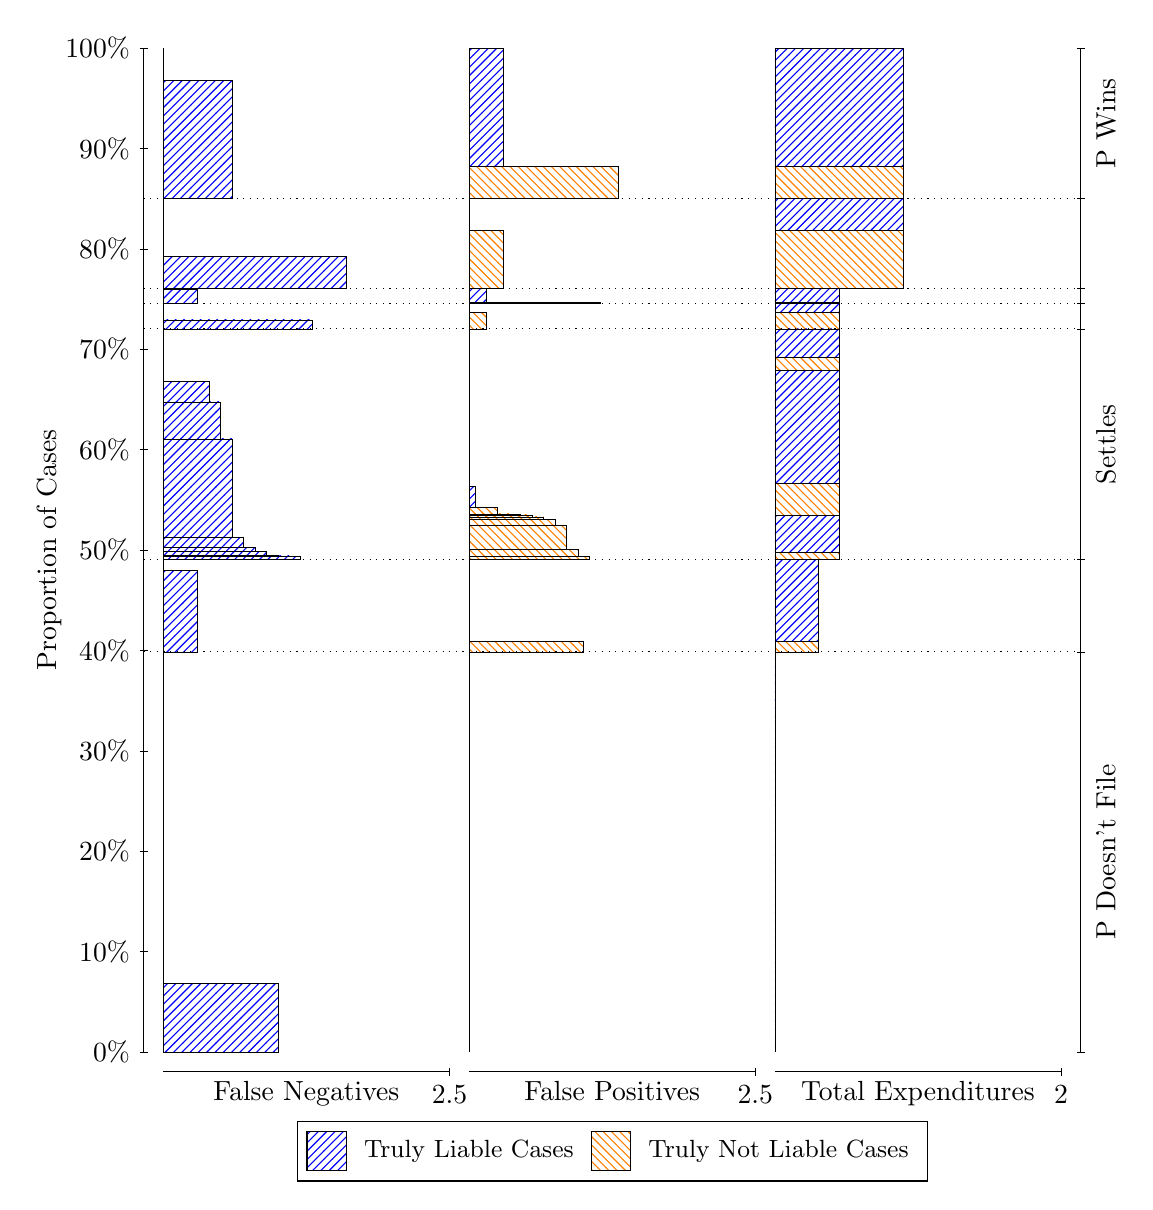
\begin{tikzpicture}
\draw[black, very thin] (1.5,1.75) -- (1.5,14.5);
\node[rotate=90, text=black, anchor=center] at (0.3, 8.125) {Proportion of Cases};
\draw[black, very thin] (1.45,1.75) -- (1.55,1.75);
\node[text=black, anchor=east] at (1.45, 1.75) {0\%};
\draw[black, very thin] (1.45,3.025) -- (1.55,3.025);
\node[text=black, anchor=east] at (1.45, 3.025) {10\%};
\draw[black, very thin] (1.45,4.3) -- (1.55,4.3);
\node[text=black, anchor=east] at (1.45, 4.3) {20\%};
\draw[black, very thin] (1.45,5.575) -- (1.55,5.575);
\node[text=black, anchor=east] at (1.45, 5.575) {30\%};
\draw[black, very thin] (1.45,6.85) -- (1.55,6.85);
\node[text=black, anchor=east] at (1.45, 6.85) {40\%};
\draw[black, very thin] (1.45,8.125) -- (1.55,8.125);
\node[text=black, anchor=east] at (1.45, 8.125) {50\%};
\draw[black, very thin] (1.45,9.4) -- (1.55,9.4);
\node[text=black, anchor=east] at (1.45, 9.4) {60\%};
\draw[black, very thin] (1.45,10.675) -- (1.55,10.675);
\node[text=black, anchor=east] at (1.45, 10.675) {70\%};
\draw[black, very thin] (1.45,11.95) -- (1.55,11.95);
\node[text=black, anchor=east] at (1.45, 11.95) {80\%};
\draw[black, very thin] (1.45,13.225) -- (1.55,13.225);
\node[text=black, anchor=east] at (1.45, 13.225) {90\%};
\draw[black, very thin] (1.45,14.5) -- (1.55,14.5);
\node[text=black, anchor=east] at (1.45, 14.5) {100\%};

\draw[black, very thin] (13.4,1.75) -- (13.4,14.5);
\draw[black, very thin] (13.35,1.75) -- (13.45,1.75);
\node[anchor=west] at (13.35, 1.75) {};
\draw[black, very thin] (13.35,6.8304) -- (13.45,6.8304);
\node[anchor=west] at (13.35, 6.8304) {};
\draw[black, very thin] (13.35,8.003) -- (13.45,8.003);
\node[anchor=west] at (13.35, 8.003) {};
\draw[black, very thin] (13.35,10.933) -- (13.45,10.933);
\node[anchor=west] at (13.35, 10.933) {};
\draw[black, very thin] (13.35,11.255) -- (13.45,11.255);
\node[anchor=west] at (13.35, 11.255) {};
\draw[black, very thin] (13.35,11.45) -- (13.45,11.45);
\node[anchor=west] at (13.35, 11.45) {};
\draw[black, very thin] (13.35,12.589) -- (13.45,12.589);
\node[anchor=west] at (13.35, 12.589) {};
\draw[black, very thin] (13.35,14.5) -- (13.45,14.5);
\node[anchor=west] at (13.35, 14.5) {};

\draw[black, very thin, pattern color=blue, pattern=north east lines] (1.75,1.75) rectangle (3.2033,2.6245);
\draw[black, very thin, pattern color=orange, pattern=north west lines] (1.75,2.6245) rectangle (1.75,6.8304);
\draw[black, very thin, pattern color=blue, pattern=north east lines] (1.75,6.8304) rectangle (2.186,7.8685);
\draw[black, very thin, pattern color=orange, pattern=north west lines] (1.75,7.8685) rectangle (1.75,8.003);
\draw[black, very thin, pattern color=blue, pattern=north east lines] (1.75,8.003) rectangle (3.494,8.0442);
\draw[black, very thin, pattern color=blue, pattern=north east lines] (1.75,8.0442) rectangle (3.3487,8.0491);
\draw[black, very thin, pattern color=blue, pattern=north east lines] (1.75,8.0491) rectangle (3.2033,8.0594);
\draw[black, very thin, pattern color=blue, pattern=north east lines] (1.75,8.0594) rectangle (3.058,8.1051);
\draw[black, very thin, pattern color=blue, pattern=north east lines] (1.75,8.1051) rectangle (3.058,8.1062);
\draw[black, very thin, pattern color=blue, pattern=north east lines] (1.75,8.1062) rectangle (2.9127,8.1555);
\draw[black, very thin, pattern color=blue, pattern=north east lines] (1.75,8.1555) rectangle (2.7673,8.2838);
\draw[black, very thin, pattern color=blue, pattern=north east lines] (1.75,8.2838) rectangle (2.622,9.537);
\draw[black, very thin, pattern color=blue, pattern=north east lines] (1.75,9.537) rectangle (2.4767,10.005);
\draw[black, very thin, pattern color=blue, pattern=north east lines] (1.75,10.005) rectangle (2.3313,10.266);
\draw[black, very thin, pattern color=orange, pattern=north west lines] (1.75,10.266) rectangle (1.75,10.933);
\draw[black, very thin, pattern color=blue, pattern=north east lines] (1.75,10.933) rectangle (3.6393,11.047);
\draw[black, very thin, pattern color=orange, pattern=north west lines] (1.75,11.047) rectangle (1.75,11.255);
\draw[black, very thin, pattern color=blue, pattern=north east lines] (1.75,11.255) rectangle (2.186,11.432);
\draw[black, very thin, pattern color=orange, pattern=north west lines] (1.75,11.432) rectangle (1.75,11.45);
\draw[black, very thin, pattern color=blue, pattern=north east lines] (1.75,11.45) rectangle (4.0753,11.856);
\draw[black, very thin, pattern color=orange, pattern=north west lines] (1.75,11.856) rectangle (1.75,12.589);
\draw[black, very thin, pattern color=blue, pattern=north east lines] (1.75,12.589) rectangle (2.622,14.09);
\draw[black, very thin, pattern color=orange, pattern=north west lines] (1.75,14.09) rectangle (1.75,14.5);
\draw[black, very thin, pattern color=orange, pattern=north west lines] (5.6333,1.75) rectangle (5.6333,5.9559);
\draw[black, very thin, pattern color=blue, pattern=north east lines] (5.6333,5.9559) rectangle (5.6333,6.8304);
\draw[black, very thin, pattern color=orange, pattern=north west lines] (5.6333,6.8304) rectangle (7.0867,6.9648);
\draw[black, very thin, pattern color=blue, pattern=north east lines] (5.6333,6.9648) rectangle (5.6333,8.003);
\draw[black, very thin, pattern color=orange, pattern=north west lines] (5.6333,8.003) rectangle (7.1593,8.0441);
\draw[black, very thin, pattern color=orange, pattern=north west lines] (5.6333,8.0441) rectangle (7.014,8.1355);
\draw[black, very thin, pattern color=orange, pattern=north west lines] (5.6333,8.1355) rectangle (6.8687,8.4418);
\draw[black, very thin, pattern color=orange, pattern=north west lines] (5.6333,8.4418) rectangle (6.7233,8.513);
\draw[black, very thin, pattern color=orange, pattern=north west lines] (5.6333,8.513) rectangle (6.578,8.5448);
\draw[black, very thin, pattern color=orange, pattern=north west lines] (5.6333,8.5448) rectangle (6.4327,8.5458);
\draw[black, very thin, pattern color=orange, pattern=north west lines] (5.6333,8.5458) rectangle (6.4327,8.5712);
\draw[black, very thin, pattern color=orange, pattern=north west lines] (5.6333,8.5712) rectangle (6.2873,8.5794);
\draw[black, very thin, pattern color=orange, pattern=north west lines] (5.6333,8.5794) rectangle (6.142,8.5824);
\draw[black, very thin, pattern color=orange, pattern=north west lines] (5.6333,8.5824) rectangle (5.9967,8.6697);
\draw[black, very thin, pattern color=blue, pattern=north east lines] (5.6333,8.6697) rectangle (5.706,8.9309);
\draw[black, very thin, pattern color=blue, pattern=north east lines] (5.6333,8.9309) rectangle (5.6333,10.933);
\draw[black, very thin, pattern color=orange, pattern=north west lines] (5.6333,10.933) rectangle (5.8513,11.141);
\draw[black, very thin, pattern color=blue, pattern=north east lines] (5.6333,11.141) rectangle (5.6333,11.255);
\draw[black, very thin, pattern color=orange, pattern=north west lines] (5.6333,11.255) rectangle (7.3047,11.272);
\draw[black, very thin, pattern color=blue, pattern=north east lines] (5.6333,11.272) rectangle (5.8513,11.45);
\draw[black, very thin, pattern color=orange, pattern=north west lines] (5.6333,11.45) rectangle (6.0693,12.182);
\draw[black, very thin, pattern color=blue, pattern=north east lines] (5.6333,12.182) rectangle (5.6333,12.589);
\draw[black, very thin, pattern color=orange, pattern=north west lines] (5.6333,12.589) rectangle (7.5227,12.999);
\draw[black, very thin, pattern color=blue, pattern=north east lines] (5.6333,12.999) rectangle (6.0693,14.5);
\draw[black, very thin, pattern color=orange, pattern=north west lines] (9.5167,1.75) rectangle (9.5167,5.9559);
\draw[black, very thin, pattern color=blue, pattern=north east lines] (9.5167,5.9559) rectangle (9.5167,6.8304);
\draw[black, very thin, pattern color=orange, pattern=north west lines] (9.5167,6.8304) rectangle (10.062,6.9648);
\draw[black, very thin, pattern color=blue, pattern=north east lines] (9.5167,6.9648) rectangle (10.062,8.003);
\draw[black, very thin, pattern color=orange, pattern=north west lines] (9.5167,8.003) rectangle (10.334,8.0943);
\draw[black, very thin, pattern color=blue, pattern=north east lines] (9.5167,8.0943) rectangle (10.334,8.5625);
\draw[black, very thin, pattern color=orange, pattern=north west lines] (9.5167,8.5625) rectangle (10.334,8.9728);
\draw[black, very thin, pattern color=blue, pattern=north east lines] (9.5167,8.9728) rectangle (10.334,10.405);
\draw[black, very thin, pattern color=orange, pattern=north west lines] (9.5167,10.405) rectangle (10.334,10.57);
\draw[black, very thin, pattern color=blue, pattern=north east lines] (9.5167,10.57) rectangle (10.334,10.933);
\draw[black, very thin, pattern color=orange, pattern=north west lines] (9.5167,10.933) rectangle (10.334,11.141);
\draw[black, very thin, pattern color=blue, pattern=north east lines] (9.5167,11.141) rectangle (10.334,11.255);
\draw[black, very thin, pattern color=orange, pattern=north west lines] (9.5167,11.255) rectangle (10.334,11.272);
\draw[black, very thin, pattern color=blue, pattern=north east lines] (9.5167,11.272) rectangle (10.334,11.45);
\draw[black, very thin, pattern color=orange, pattern=north west lines] (9.5167,11.45) rectangle (11.152,12.182);
\draw[black, very thin, pattern color=blue, pattern=north east lines] (9.5167,12.182) rectangle (11.152,12.589);
\draw[black, very thin, pattern color=orange, pattern=north west lines] (9.5167,12.589) rectangle (11.152,12.999);
\draw[black, very thin, pattern color=blue, pattern=north east lines] (9.5167,12.999) rectangle (11.152,14.5);
\draw[black, dotted] (1.5,6.8304) -- (13.4,6.8304);
\draw[black, dotted] (1.5,8.003) -- (13.4,8.003);
\draw[black, dotted] (1.5,10.933) -- (13.4,10.933);
\draw[black, dotted] (1.5,11.255) -- (13.4,11.255);
\draw[black, dotted] (1.5,11.45) -- (13.4,11.45);
\draw[black, dotted] (1.5,12.589) -- (13.4,12.589);
\draw[black, very thin] (1.75,1.5) -- (5.3833,1.5);
\node[text=black, anchor=north] at (3.5667, 1.5) {False Negatives};
\draw[black, very thin] (5.3833,1.45) -- (5.3833,1.55);
\node[text=black, anchor=north] at (5.3833, 1.45) {2.5};

\draw[black, very thin] (5.6333,1.5) -- (9.2667,1.5);
\node[text=black, anchor=north] at (7.45, 1.5) {False Positives};
\draw[black, very thin] (9.2667,1.45) -- (9.2667,1.55);
\node[text=black, anchor=north] at (9.2667, 1.45) {2.5};

\draw[black, very thin] (9.5167,1.5) -- (13.15,1.5);
\node[text=black, anchor=north] at (11.333, 1.5) {Total Expenditures};
\draw[black, very thin] (13.15,1.45) -- (13.15,1.55);
\node[text=black, anchor=north] at (13.15, 1.45) {2};

\node[text=black, centered, rotate=90] at (13.72, 4.2902) {P Doesn't File};

\node[text=black, centered, rotate=90] at (13.72, 9.4681) {Settles};



\node[text=black, centered, rotate=90] at (13.72, 13.544) {P Wins};

\draw (7.449999999999999,1.5) node[draw=none] (baseCoordinate) {};
\begin{scope}[align=center]
        \matrix[scale=0.5, draw=black, below=0.5cm of baseCoordinate, nodes={draw}, column sep=0.1cm]{
            \node[rectangle, draw, minimum width=0.5cm, minimum height=0.5cm, pattern color=blue, pattern=north east lines] {}; &
            \node[draw=none, font=\small, text=black] (B) {Truly Liable Cases}; &
            \node[rectangle, draw, minimum width=0.5cm, minimum height=0.5cm, pattern color=orange, pattern=north west lines] {}; &
            \node[draw=none, font=\small, text=black] (B) {Truly Not Liable Cases}; \\
            };
\end{scope}

\end{tikzpicture}
\end{document}